\documentclass[12pt,twoside]{article} \usepackage{light}
\usepackage{subfigure} \usepackage{graphicx}
%\hidesolutions
\showsolutions

\begin{document}

\problemset{4}{September 28, 2010}{Monday, October 4 (7pm)}
\begin{problem}{15}
Let $G = (V,E)$ be a graph. A {\em matching} in $G$ is a set $M
\subset E$ such that no two edges in $M$ are incident on a common
vertex.

Let $M_1$, $M_2$ be two matchings of $G$. Consider the new graph $G' =
(V, M_1 \cup M_2)$ (i.e. on the same vertex set, whose edges consist
of all the edges that appear in either $M_1$ or $M_2$). Show that $G'$
is bipartite.

{\em Helpful definition}: A {\em connected component} is a subgraph of
a graph consisting of some vertex and every node and edge that is
connected to that vertex.

\solution{
\begin{proof}

Proof by induction on the number of vertices $n$:

\textbf{Induction hypothesis:} $P(n)$ is defined to be: Let $G$ be a
graph with $n$ vertices and matchings $M_1$ and $M_2$. Let $G' = (V,
M_1 \cup M_2)$. Then $G'$ is bipartite.

\textbf{Base case:} $G$ has only one vertex and so is bipartite.
$P(1)$ holds.

\textbf{Inductive step:} We will assume $P(n)$ in order to prove
$P(n+1)$.

Let $G$ be a graph with $n+1$ vertices.  We will remove a vertex $v$
from $G$ to obtain an $n$ vertex graph, $G_1$, with vertex set
$V_1$. If we remove $v$ we will be in one of the following cases:


\textbf{Case 1:} $v$ is in none of the edges in $M_1$ nor $M_2$.

By our inductive hypothesis we know that since $G_1$ has $n$ vertices
and $M_1$ and $M_2$ are matchings of $G_1$, then $G_1'=(V_1, M_1 \cup
M_2)$ is bipartite. Since $G_1'$ is bipartite, there exists a
partition of the vertices into two sets, $L$ and $R$ such that every
edge is incident to a vertex in $L$ and to a vertex in $R$. We can now
add $v$ to either set and obtain a bipartite representation of $G'$.

\textbf{Case 2:} $v$ is in an edge in either $M_1$ or $M_2$, we will
assume, without loss of generality, that $v$ is in an edge in $M_1$.

Suppose the edge $v-x$ is in $M_1$, now remove $v-x$ from $M_1$ to
obtain $M_1'$.

Now by our inductive hypothesis we know that since $G_1$ has $n$
vertices and $M_1'$ and $M_2$ are matchings of $G_1$, then $G_1'=(V_1,
M_1' \cup M_2)$ is bipartite. Since $G_1'$ is bipartite, there exists
a partition of the vertices into two sets, $L$ and $R$ such that every
edge is incident to a vertex in $L$ and to a vertex in $R$.

We know that the vertex $x$ is in either $L$ or $R$. We can just add
vertex $v$ to the other set, along with edge $v-x$, and we obtain a
valid partitioning of $L$ and $R$ for our graph $G'$.



\textbf{Case 3:} $v$ is in both $M_1$ and $M_2$

Suppose the edge $v-x$ is in $M_1$ and $v-y$ is in $M_2$, now remove
those edges from $M_1$ and $M_2$ to obtain $M_1'$ and $M_2'$.

Now by our inductive hypothesis we know that since $G_1$ has $n$
vertices and $M_1'$ and $M_2'$ are matchings of $G_1$, then
$G_1'=(V_1, M_1' \cup M_2')$ is bipartite. Since $G_1'$ is bipartite,
there exists a partition of the vertices into two sets, $L$ and $R$
such that every edge is incident to a vertex in $L$ and to a vertex in
$R$.

If $x$ and $y$ in the same set, either $L$ or $R$, then we can just
add $v$ to the other set, and add edges $v-x$ and $v-y$ to obtain
$G'$. So our graph remains bipartite.

If $x$ and $y$ are on different sides of $L$ and $R$, then either $x$
and $y$ are in the same connected component or they are in different
connected components. If $x$ and $y$ are in different connected
components, then each connected component has a corresponding set of
$L$ and $R$ vertices, such that there are edges only within that
component. Let's say that the first component has left and right
vertices in the set $L_1$ and $R_1$, and the second component has sets
$L_2$ and $R_2$, where $L=L_1 \cup L_2$ and $R=R_1 \cup R_2$. Now if
we swap $L_1$ and $R_1$ -- that is we define $L=R_1 \cup L_2$ and
$R=L_1 \cup R_2$ -- then our graph will remain bipartite, as there
were edges only within the connected components. But after the
swapping $x$ and $y$ will be in the same set, $L$ or $R$, and as
before we can just add $v$ to the other set to get a bipartite graph
for $G'$ as desired.

Now we will show that it is impossible for $x$ and $y$ to be on
opposite sides and in the same component.

Suppose for a contradiction that $x$ and $y$ are in the same connected
component and $x$ and $y$ are both in $L$. Then since they are in the
same connected component there is a path from $x$ to $y$ say $x-v_1,
v_1-v_2, \ldots, v_k-y$, where $k$ is even. Then the edges $x-v_1$ and
$v_2-v_3$, $v_4-v_5, \ldots, v_k-y$ must all be in the same matching
(otherwise we will have two edges incident on the same vertex in the
same matching). This is a contradiction since our original $M_1$
cannot have any edge with $x$ and $M_2$ cannot have any edge with $y$
(since a matching has only one edge incident to a vertex). So this
cannot be the case and $x$ and $y$ must be on the same side.

Hence we conclude that in all cases $G'$ is bipartite.

Therefore by induction our claim holds.
\end{proof}

}
\end{problem}

\begin{problem}{20}
Let $G = (V,E)$ be a graph. Recall that the {\em degree} of a vertex
$v \in V$, denoted $d_v$, is the number of vertices $w$ such that
there is an edge between $v$ and $w$.  \bparts \ppart{10} Prove
that $$2|E| = \sum_{v\in V} d_v.$$ \solution{ Let $S = \{(e,v) \in E
  \times V: e \mbox{ is incident on } v\}$.

Count the elements in $S$ as follows
$$|S| = \sum_{e \in E} |\{v: (e,v) \in S\}| = 2 |E|$$ and also as
$$ |S| = \sum_{v \in V} |\{e: (e,v) \in S\}| = \sum_{v\in V} d_v.$$
The result follows.

Once can also prove it by induction on $|E|$. You should try to.  }
\ppart{5} At a 6.042 ice cream study session (where the ice cream is
plentiful and it helps you study too) 111 students showed up. During
the session, some students shook hands with each other (everybody
being happy and content with the ice-cream and all). Turns out that
the University of Chicago did another spectacular study here, and
counted that each student shook hands with exactly 17 other
students. Can you debunk this too?  \solution{ Assume that the study
  is accurate. Define a graph $G=(V,E)$ with students as vertices and
  put an edge between 2 students if they shook hands. By the previous
  problem, we should have $2|E| = \sum_{v} d_v = 111\cdot 17$. But the
  LHS is even and the RHS is odd, a contradiction.}  \ppart{5} And on
a more dull note, how many edges does $K_n$, the complete graph on $n$
vertices, have?  \solution{ Apply the first part of the
  problem. Notice that each vertex is joined to $n-1$ others.  $2|E| =
  \sum_{v}d_v = n(n-1)$. So $|E| = n(n-1)/2$.}  \eparts

\end{problem}

\begin{problem}{15}
Two graphs are isomorphic if they are the same up to a relabeling of
their vertices (see Definition 5.1.3 in the book). A property of a
graph is said to be \emph{preserved under isomorphism} if whenever $G$
has that property, every graph isomorphic to $G$ also has that
property.  For example, the property of having five vertices is
preserved under isomorphism: if $G$ has five vertices then every graph
isomorphic to $G$ also has five vertices.

\bparts \ppart{5} Some properties of a simple graph, $G$, are
described below. Which of these properties is {\em preserved under
  isomorphism}?

\begin{enumerate}
\item
$G$ has an even number of vertices.

\item
None of the vertices of $G$ is an even integer.

\item
$G$ has a vertex of degree 3.

\item
$G$ has exactly one vertex of degree 3.

\end{enumerate}

\solution{
\begin{enumerate}
\item It is invariant under isomorphism. There must be an one-to-one
  and onto mapping between the vertices of two isomorphic
  graphs. Therefore, the number of vertices in the two graphs must be
  the same. If one graph has even number of vertices, then the other
  must have even number of vertices.

\item
 It is not invariant under isomorphism. We do not really care what the
 vertices are. Vertices can be any kind of mathematical objects.  All
 we are interested is that whether there exists a one-to-one and onto
 function $f$ mapping from vertices of one graph to vertices of
 another with the property that $a$ and $b$ are adjacent in the first
 graph if and only if $f(a)$ and $f(b)$ are adjacent in the second
 graph, for all $a$ and $b$ in the first graph. \\

So, for example, let $G_1$ be a graph with a single vertex, 1, and
$G_2$ be a graph with a single vertex, 2. Obviously the two graphs are
isomorphic, but $G_2$ does not have vertices which are even integers.

\item
 It is invariant under isomorphism.

Let $G_1, G_2$ be simple graphs and $f:V_1\to V_2$ be an isomorphism
between them.  Suppose $v\in V_1$ has degree 3; we want to show that
there is a vertex of degree 3 in $V_2$.  In fact, we'll show that
$f(v)$ has degree 3.
 
Since $v$ has degree 3, there are exactly 3 vertices adjacent to $v$;
say these are $v_1,v_2,v_3$.  Since $f$ is a bijection,
$f(v_1),f(v_2)$ and $f(v_3)$ are all distinct.  Since there is an edge
between $v$ and $v_i$ in $G_1$, the definition of isomrphism implies
that there is an edge between $f(v)$ and $f(v_i)$ for $i=1,2,3$, so
the degree of $f(v)$ is at least 3.
 
We now prove by contradiction that the degree of $f(v)$ is at most 3.
Suppose $f(v)$ had degree $>3$.  This means there is a vertex $w \in
V_2$ which is not equal to $f(v_1), f(v_2),$ or $f(v_3)$, but is also
adjacent to $f(v)$.  Since, $f$ is a bijection, there is a vertex $v_4
\in V_1$ such that $f(v_4) = w$ and $v_4 \neq v_i$ for $i=1,2,3$.
Since $w=f(v_4)$ is adjacent to $f(v)$, the definition of isomorphism
implies that $v_4$ is adjacent to $v$, contradicting the fact the
$v_1,v_2,v_3$ were exactly the vertices adjacent to $v$.

\item
  It is invariant under isomorphism.

Prove by contradiction: Suppose a graph $G_1$ has exactly one vertex
of degree $3$ while another graph $G_2$ does not have exactly one
vertex of degree 3. Suppose the two graphs are isomorphic. If $G_2$
does not have a vertex of degree 3, then from part (c), there is a
contradiction.  If $G_2$ has more than one vertices of degree 3, then
there must be at least one vertex in $G_2$ of degree 3 which is mapped
to a vertex of degree $\neq 3$ in $G_1$. Since two vertices of
different degrees are mapped from $G_1$ to $G_2$, using the same
argument from part (c), it reaches a contradiction. Therefore, if
$G_1$ has exactly one vertex of degree 3, then $G_2$ must also have
exactly one vertex of degree 3.

\end{enumerate}

} \ppart{10} Determine which among the four graphs pictured in the
Figures
%~\ref{fig:isog}
are isomorphic.  If two of these graphs are isomorphic, describe an
isomorphism between them.  If they are not, give a property that is
preserved under isomorphism such that one graph has the property, but
the other does not.  For at least one of the properties you choose,
\emph{prove} that it is indeed preserved under isomorphism (you only
need prove one of them).

\begin{figure}[h] %[htbp]
\begin{center}
\mbox{ \subfigure[$G_1$]{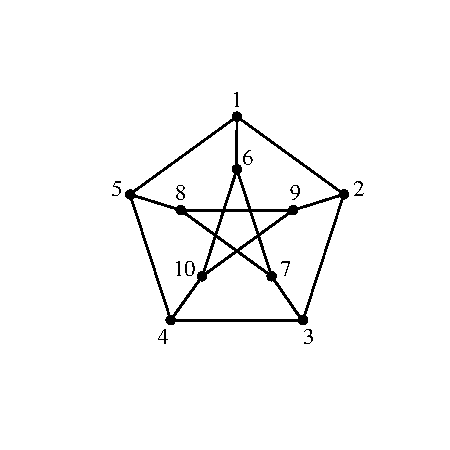
\includegraphics[width=1.5in,clip]{G1}}
        \hspace{17mm}
        \subfigure[$G_2$]{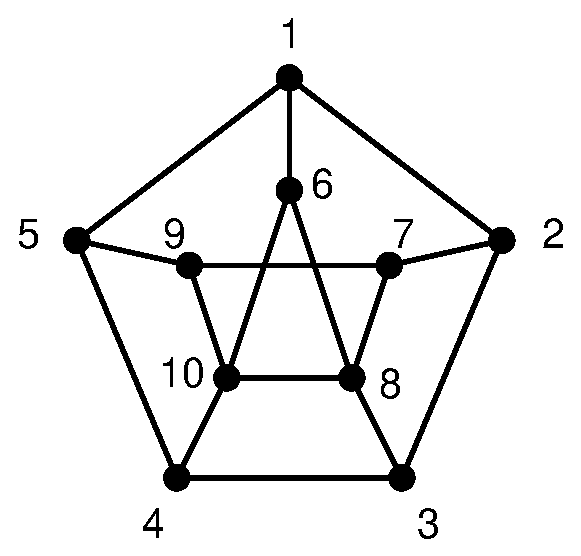
\includegraphics[width=1.5in,clip]{G4}} }
\mbox{ \subfigure[$G_3$]{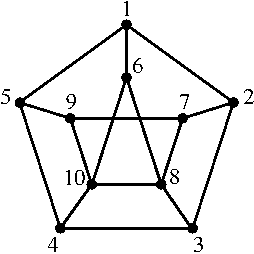
\includegraphics[width=1.5in,clip]{G2}}
        \hspace{17mm}
        \subfigure[$G_4$]{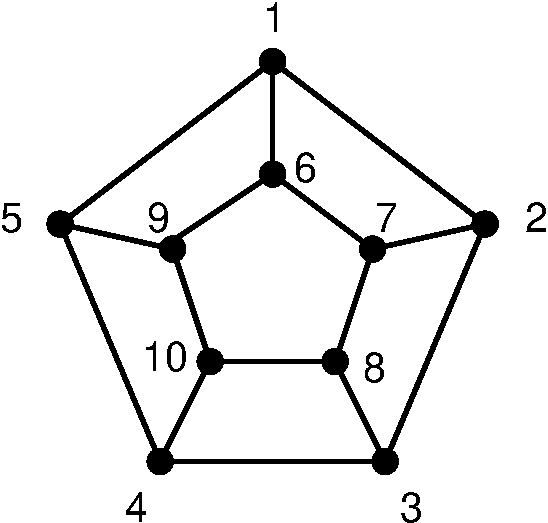
\includegraphics[width=1.5in,clip]{G3}} }
\end{center}
\caption{Which graphs are isomorphic?}
\label{fig:isog}
\end{figure}

\iffalse

\begin{figure}[h] %[htbp]
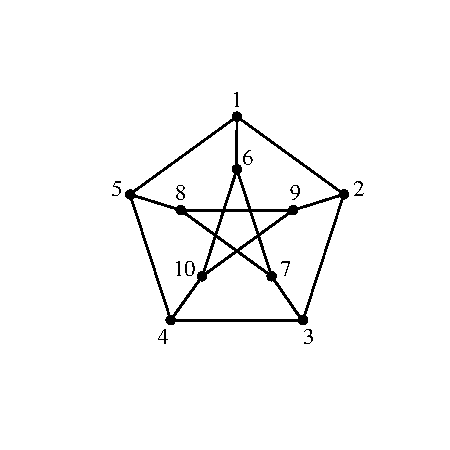
\includegraphics[width=1.5in,clip]{G1}
\caption{$G_1$}
\label{fig:G1}
\end{figure}

\begin{figure}[h] %[htbp]
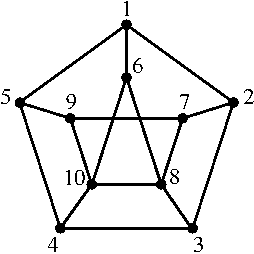
\includegraphics[width=1.5in,clip]{G2}
\caption{$G_2$}
\label{fig:G2}
\end{figure}

\begin{figure}[h] %[htbp]
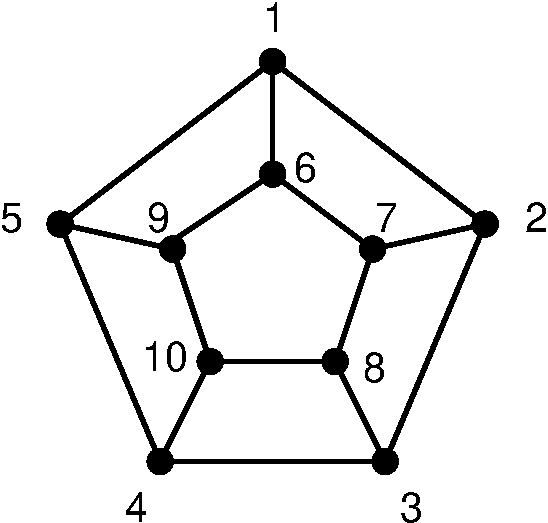
\includegraphics[width=1.5in,clip]{G3}
\caption{$G_3$}
\label{fig:G3}
\end{figure}

\begin{figure}[h] %[htbp]
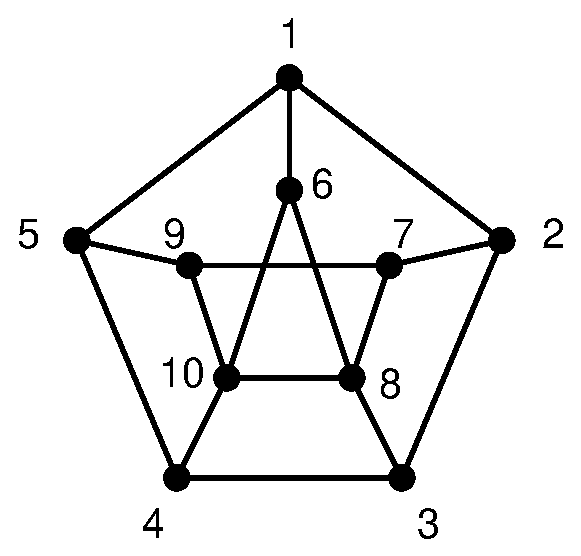
\includegraphics[width=1.5in,clip]{G4}
\caption{$G_4$}
\label{fig:G4}
\end{figure}
\fi

\solution{ $G_1$ and $G_3$ are isomorphic.  In particular, the
  function $f:V_1 \to V_3$ is an isomomorphism, where
\begin{align*}
&f(1)=1 \quad&& f(2)=2 \quad&& f(3)=3 \quad&& f(4)=8 \quad&& f(5)=9
  \\ &f(6)=10 \quad&& f(7)=4 \quad&& f(8)=5 \quad&& f(9)=6 \quad&&
  f(10)=7
\end{align*}

$G_1$ and $G_4$ are not isomorphic to $G_2$: $G_2$ has a vertex of
degree four and neither $G_1$ nor $G_4$ has one.

$G_1$ and $G_4$ are not isomorphic: $G_4$ has a simple cycle of length
four and $G_1$ does not.

} \eparts

\end{problem}

\begin{problem}{15}
Recall that a \term{coloring} of a simple graph is an assignment of a
color to each vertex such that no two adjacent vertices have the same
color.  A \term{$k$-coloring} is a coloring that uses at most $k$
colors.

\begin{falseclm*}
Let $G$ be a (simple) graph with maximum degree at most $k$.  If $G$
also has a vertex of degree less than $k$, then $G$ is $k$-colorable.
\end{falseclm*}

\bparts \ppart{5}\label{counterexample} Give a counterexample to the
False Claim when $k=2$.

\solution{One node by itself, and a separate triangle ($K_3$).  The
  graph has max degree 2, and a node of degree zero, but is not
  2-colorable.}

\ppart{10} Consider the following proof of the False Claim:

\begin{proof}

Proof by induction on the number $n$ of vertices:

{\bf Induction hypothesis:} $P(n)$ is defined to be: Let $G$ be a
graph with $n$ vertices and maximum degree a most $k$.  If $G$ also
has a vertex of degree less than $k$, then $G$ is $k$-colorable.

{\bf Base case:} (n=1) $G$ has only one vertex and so is 1-colorable.
So $P(1)$ holds.

{\bf Inductive step:}

We may assume $P(n)$.  To prove $P(n+1)$, let $G_{n+1}$ be a graph
with $n+1$ vertices and maximum degree at most $k$.  Also, suppose
$G_{n+1}$ has a vertex, $v$, of degree less than $k$.  We need only
prove that $G_{n+1}$ is $k$-colorable.

To do this, first remove the vertex $v$ to produce a graph, $G_n$,
with $n$ vertices.  Removing $v$ reduces the degree of all vertices
adjacent to $v$ by 1.  So in $G_n$, each of these vertices has degree
less than $k$.  Also the maximum degree of $G_n$ remains at most $k$.
So $G_n$ satisfies the conditions of the induction hypothesis $P(n)$.
We conclude that $G_n$ is $k$-colorable.

Now a $k$-coloring of $G_n$ gives a coloring of all the vertices of
$G_{n+1}$, except for $v$.  Since $v$ has degree less than $k$, there
will be fewer than $k$ colors assigned to the nodes adjacent to $v$.
So among the $k$ possible colors, there will be a color not used to
color these adjacent nodes, and this color can be assigned to $v$ to
form a $k$-coloring of $G_{n+1}$.
\end{proof}

Identify the exact sentence where the proof goes wrong.\\

\solution{``So $G_n$ satisfies the conditions of the induction
  hypothesis $P(n)$.''  The flaw is that if $v$ has degree 0, then
  removing $v$ will not reduce the degree of any vertex, and so there
  may not be any vertex of degree less than $k$ in $G_n$, as in the
  counterexample of part~\eqref{counterexample}.}


\eparts
\end{problem}

\begin{problem}{15} Prove or disprove the following claim: for
some $n \geq 3$ ($n$ boys and $n$ girls, for a total of $2n$ people),
there exists a set of boys' and girls' preferences such that every
dating arrangement is stable.\\

\solution{ The claim is false.

\begin{proof} We will use letters to denote girls and numbers to denoted boys.

There must be some girl $A$ rated worst by at most $n-2$ boys.  The
reason is as follows.  Each boy can rate exactly one girl worst.  If
each of the $n$ girls was rated worst by at least $n-1$ boys, then
there would have to be at least $n (n-1)$ boys in all.  But this is
false when $n \geq 3$, because then $n (n-1)$ exceeds $n$, the actual
number of boys.

Suppose that this girl $A$ is paired with the boy, 1, that she rates
worst.  Since at most $n-2$ boys rate girl $A$ worst, there is some
other boy, 2, that rates a different girl, $B$, worst.  Suppose that
boy 2 is paired with girl $B$.

Now girl $A$ and boy $2$ form a rogue couple.  Girl $A$ prefers every
other boy to her date, 1.  Similarly, boy $2$ prefers every other girl
to his date $B$.  Therefore, $A$ and $2$ prefer one another to their
current dates.
\end{proof}
}
\end{problem}

\begin{problem}{20}

Let $(s_1, s_2, ..., s_n)$ be an arbitrarily distributed sequence of
the number $1,2,...,n-1,n$. For instance, for $n=5$, one arbitrary
sequence could be $(5, 3, 4, 2, 1)$.

Define the graph G=(V,E) as follows:

\begin{enumerate}
\item $V = \{v_1, v_2,...,v_n\}$

\item $e=(v_i, v_j) \in E$ if either:

\begin{enumerate}
\item
$j=i+1$, for $1 \leq i \leq n-1$
\item
$i=s_k$, and $j=s_{k+1}$ for $1 \leq k \leq n-1$
\end{enumerate}
\end{enumerate}

\bparts \ppart{10} Prove that this graph is 4-colorable for any $(s_1,
s_2, \ldots, s_n)$.

Hint: First show that a line graph is 2-colorable. Note that a line
graph is defined as follows: The $n$-node graph containing $n - 1$
edges in sequence is known as the line graph $L_n$.

\solution{ First we argue that any line graph is 2-colorable. Consider
  the line graph $L_n$ with vertices $v_1, v_2, v_3, \ldots,
  v_n$. Suppose we have two colors $A$ and $B$. Then color all odd
  numbered vertices with color $A$ and all even numbered vertices with
  color $B$. Since each odd vertex is adjacent only to even vertices,
  and vice versa, this is a valid 2-coloring.

Consider $G$. $G$ is composed of two---possibly overlapping---line
graphs: one line graph contains the vertices of $G$ in order, while
the other line graph of the vertices of $G$ in the order of our
sequence $(s_1, \ldots, s_n)$. Pick one of these two graphs to color
first using colors A and B.  This will be a temporary coloring. Now
color the second line graph with colors C and D, noting that these are
temporary colors as well. Now each vertex will be assigned two colors,
one from the first line graph and one from the second line graph
(since both line graphs contain all vertices). Define four new colors,
AC, AD, BC, BD. Color the graph with AC if one temporary color is A
and the other temporary color is C. Color the graph with AD if one
temporary color is A and the other is D. Do the same with colors BC
and BD.

We note that our original temporary colors represent adjacencies in
the graph. That is we note that each vertex has at most 4 adjacent
nodes (two from each line graph). If the first color is A then two of
the adjacenct vertices will be colored B, and vice versa. If the
second color is C, then the other two adjacenct vertices will be
colored D, and vice versa. So if a graph has a specific color, such as
AC, then it is adjacent only to vertices of color B and D. Since we
color those vertices differently (with one of AB, BC, or BD), then our
coloring does not color two adjacent vertices with the same color.  }

\ppart{10} Suppose $ (s_1,s_2, \ldots ,s_n)= (1,a_1,3,a_2,5,a_3,
\ldots)$ where $a_1, a_2, \ldots$ is an arbitrary distributed sequence
of the even numbers in ${1, \ldots, n-1}$. Prove that the resulting
graph is 2-colorable.

\solution{ Color all odd vertices with first color. Now color all the
  even vertices with a second color. Note that by problem definition
  odd vertices are only adjacent to even vertices and vice versa,
  hence this is a valid 2-coloring.

} \eparts
\end{problem}

\end{document}
